\chapter{Additional TC Genesis Plots}\label{sec:genesis-appendix}

\begin{figure}[ht]
	\centering
	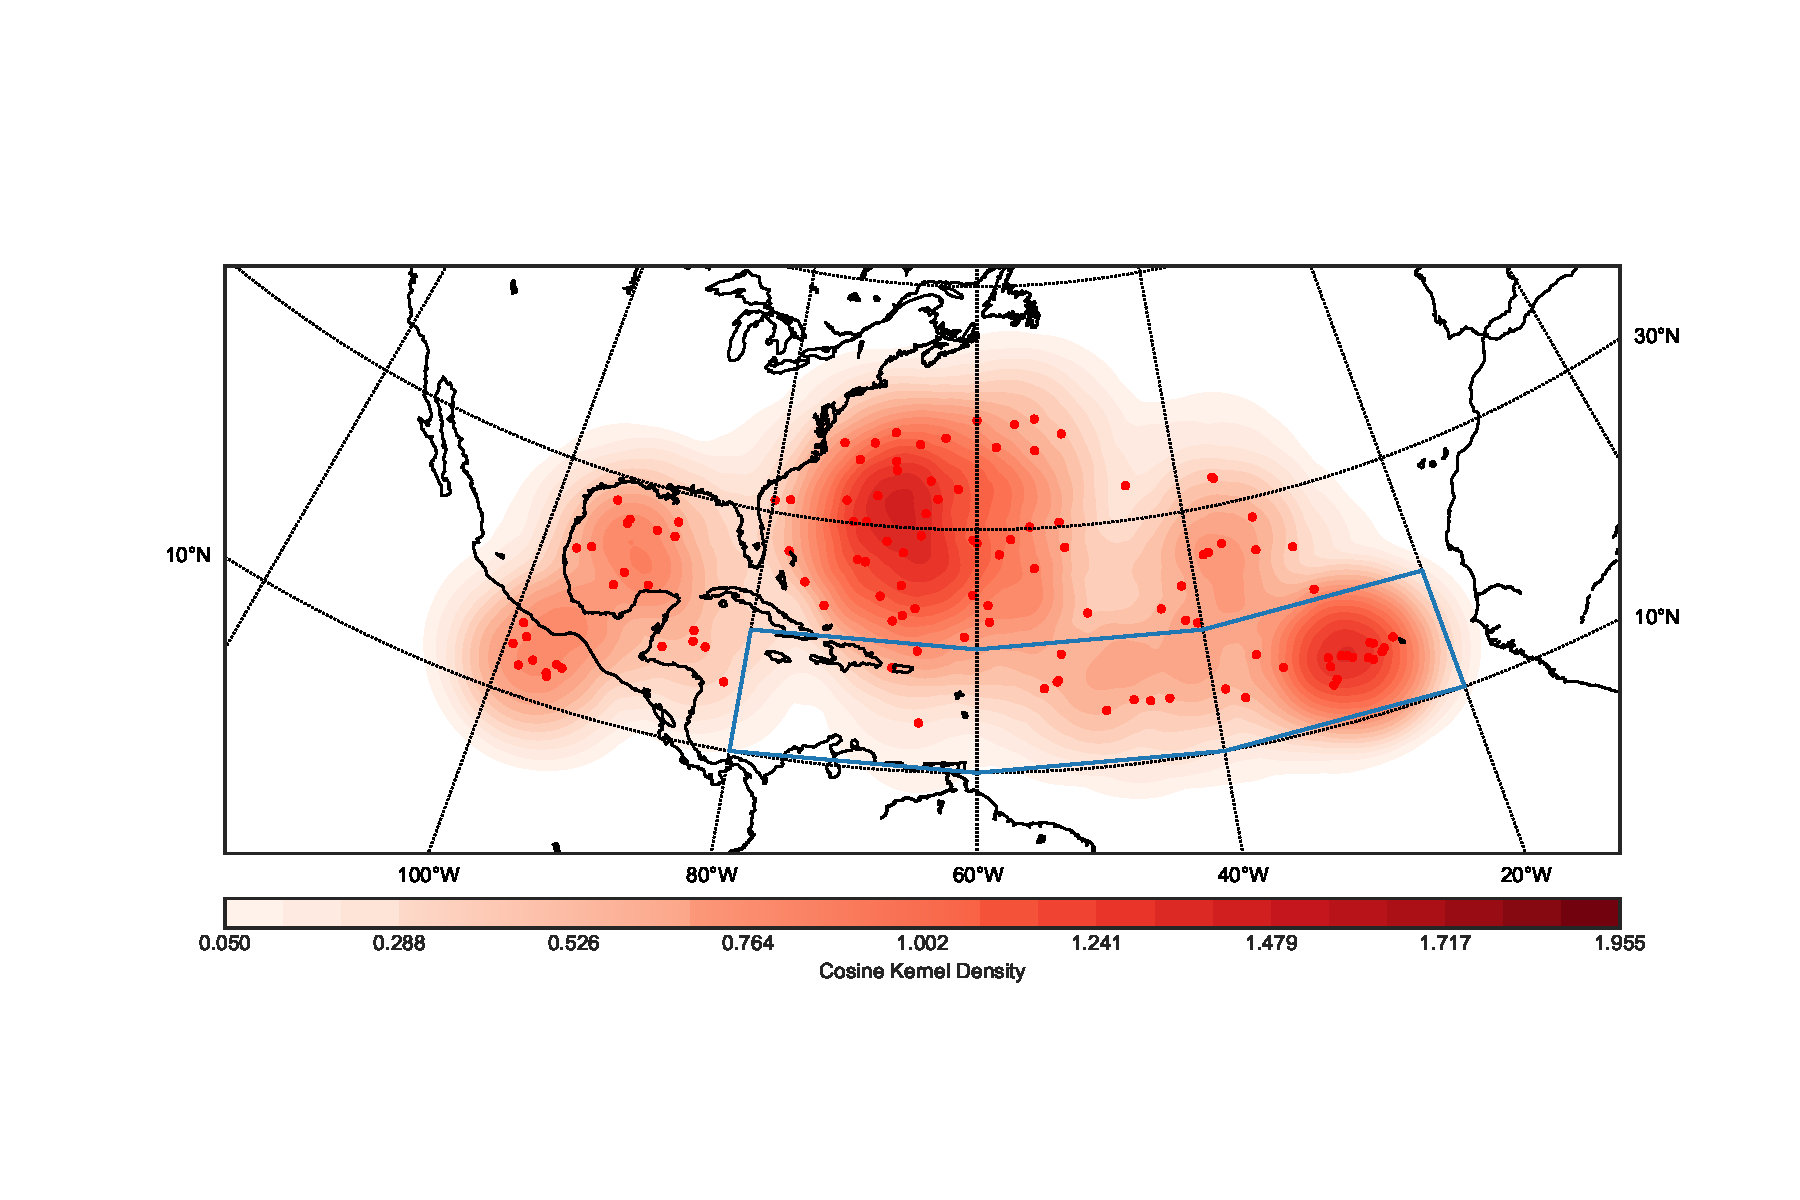
\includegraphics[width=0.8\textwidth]{img/genesis_plot_temdif05.pdf}
	\caption{Genesis spots and density for temdif = 0.5.Using param\_id = 109.}
\end{figure}
\begin{figure}[ht]
	\centering
	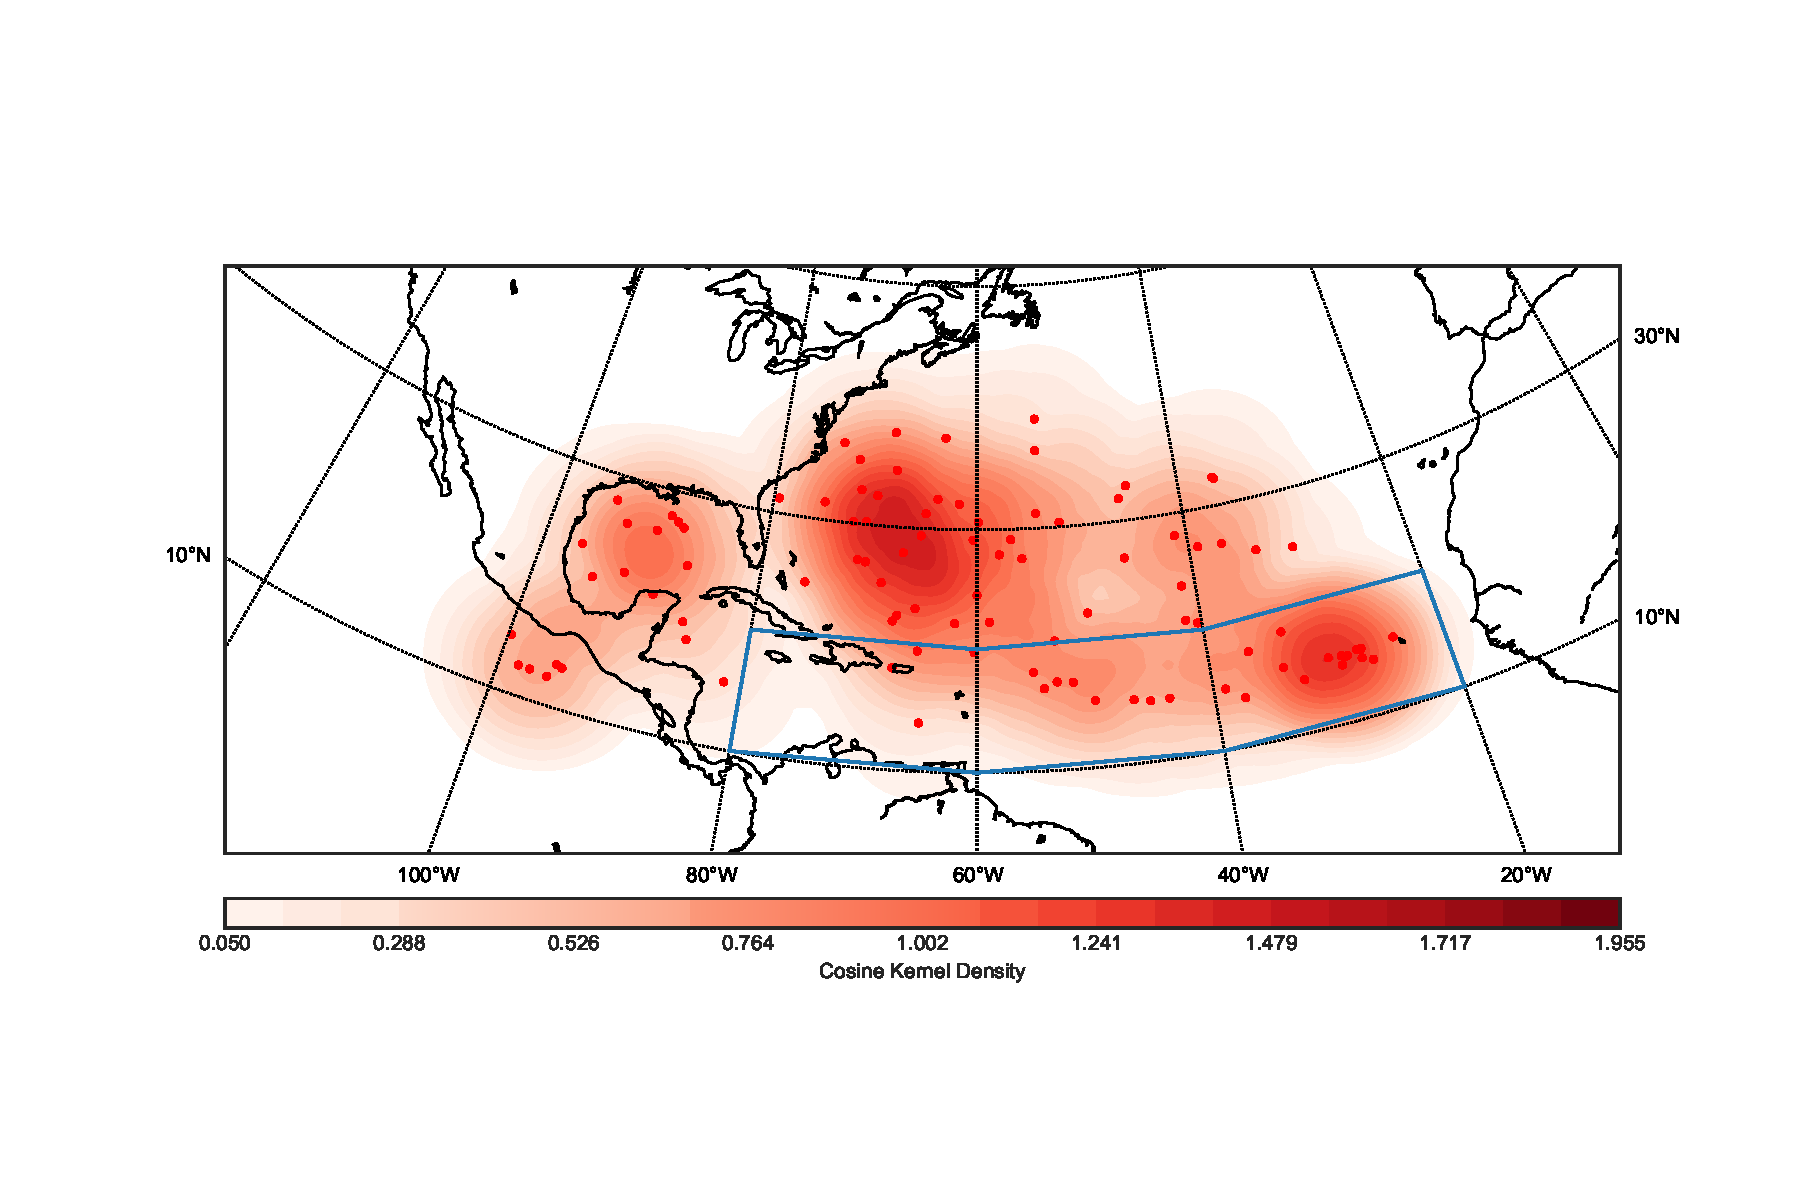
\includegraphics[width=0.8\textwidth]{img/genesis_plot_temdif075.pdf}
	\caption{Genesis spots and density for temdif = 0.75. Using param\_id = 129.}
\end{figure}
\begin{figure}[ht]
	\centering
	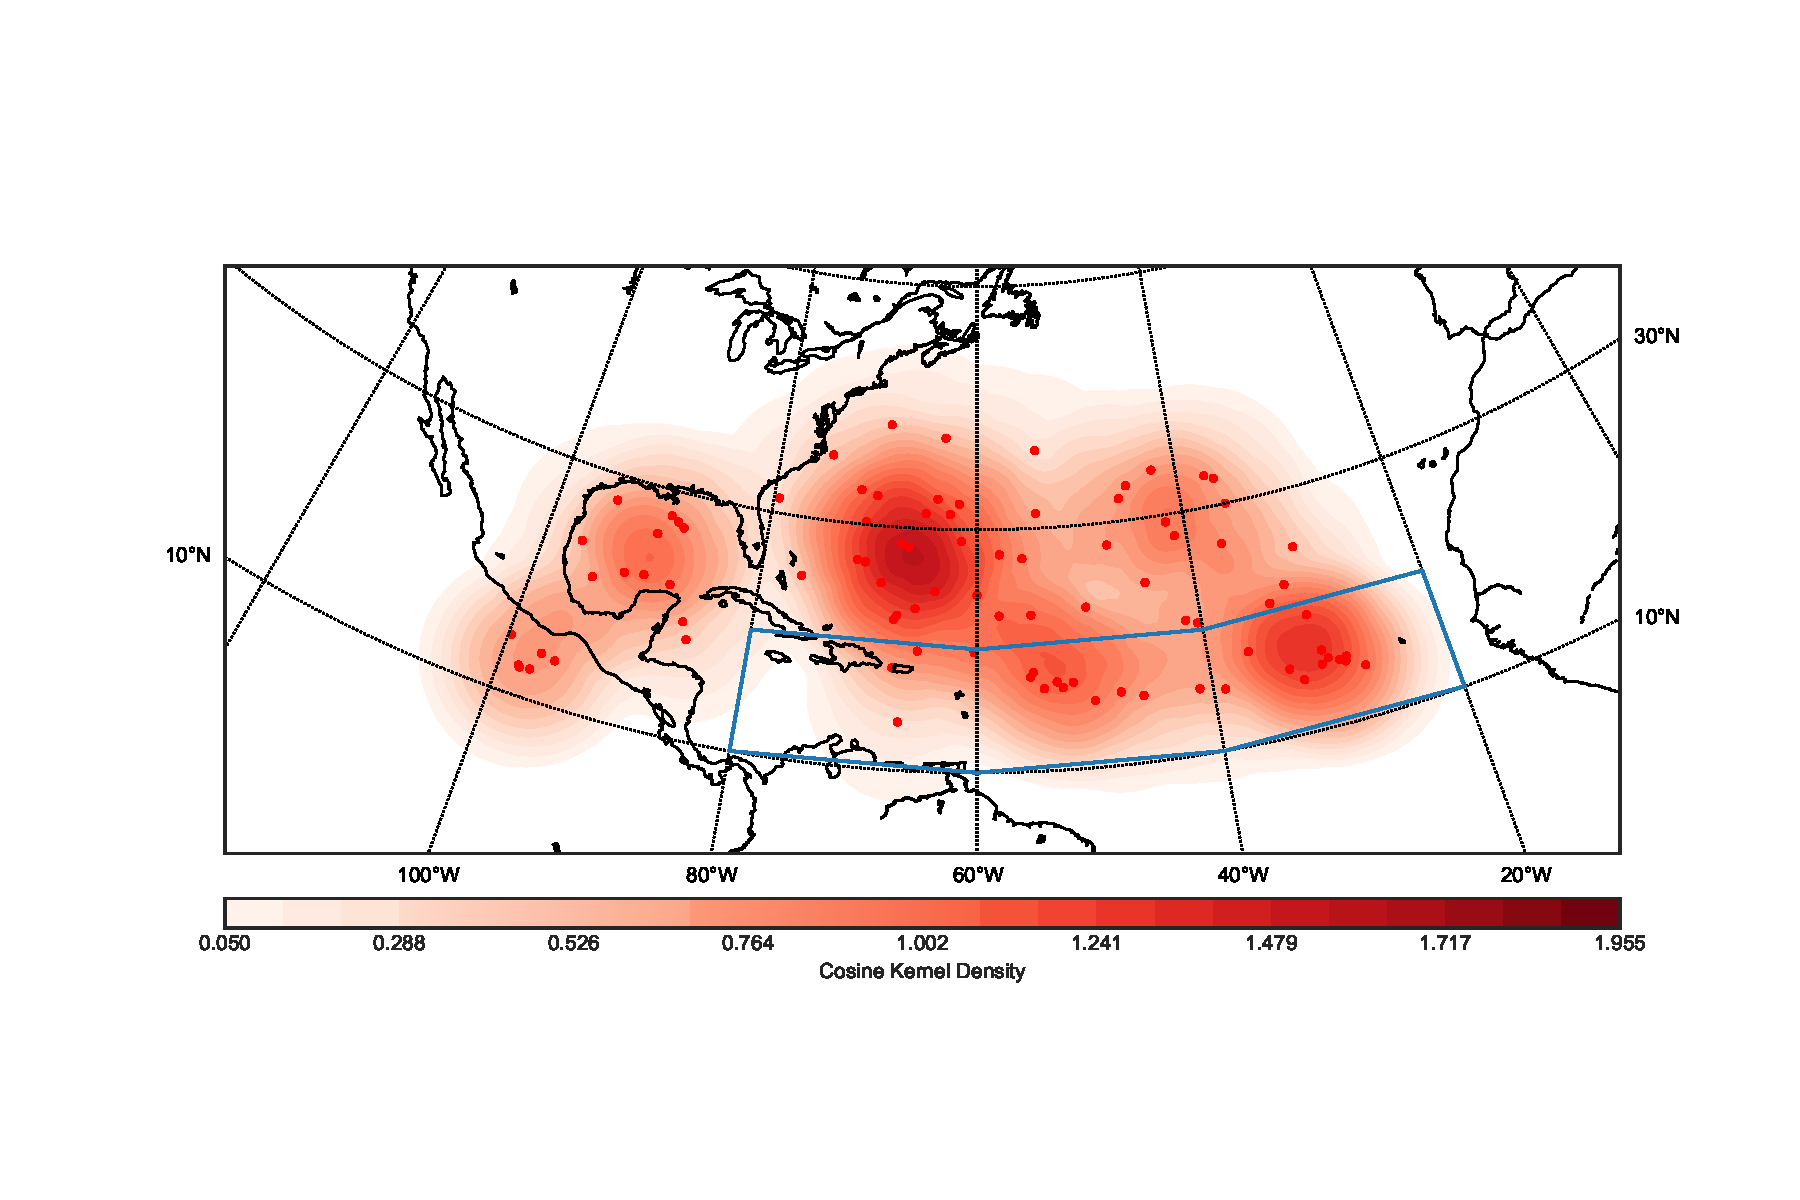
\includegraphics[width=0.8\textwidth]{img/genesis_plot_temdif1.pdf}
	\caption{Genesis spots and density for temdif = 1.0. Using param\_id = 149.}
\end{figure}
\begin{figure}[ht]
	\centering
	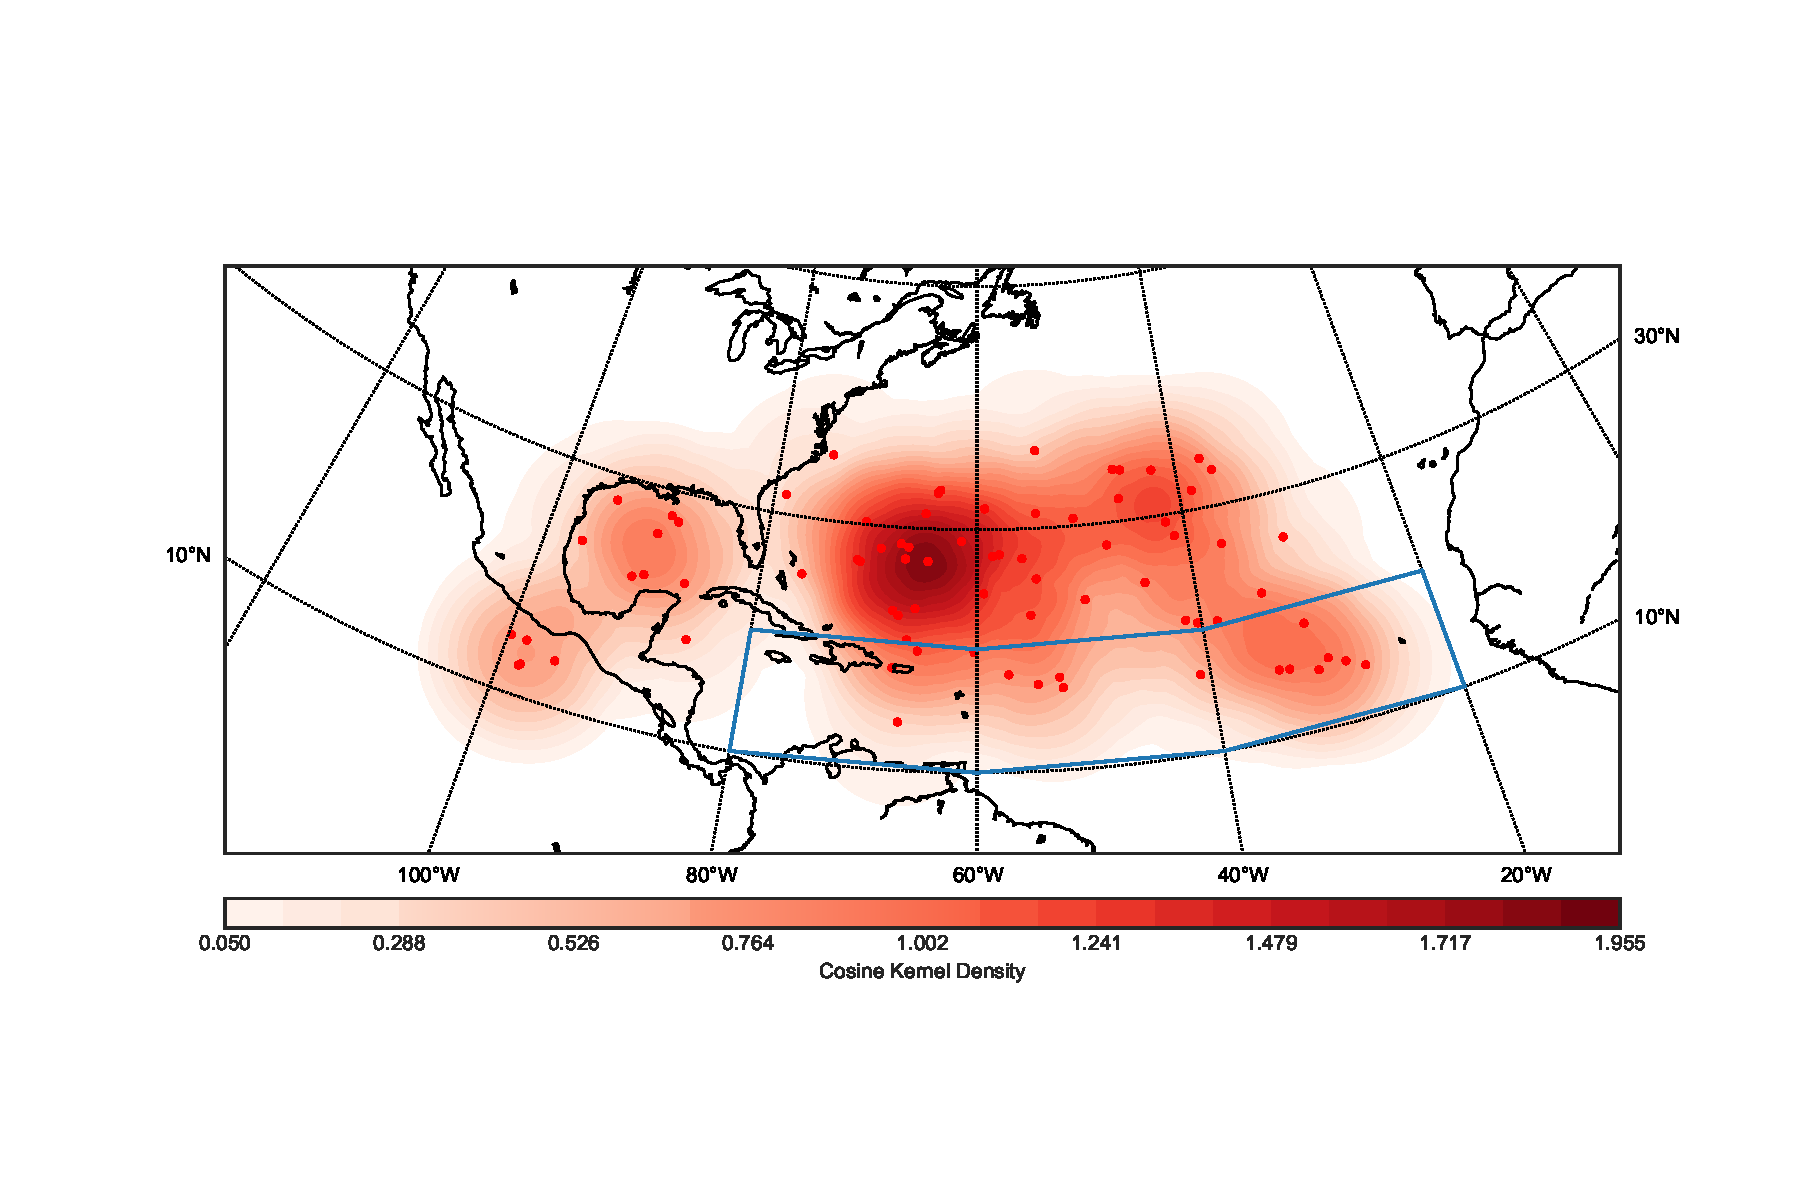
\includegraphics[width=0.8\textwidth]{img/genesis_plot_temdif125.pdf}
	\caption{Genesis spots and density for temdif = 1.25. Using param\_id = 160.}
\end{figure}
\begin{figure}[ht]
	\centering
	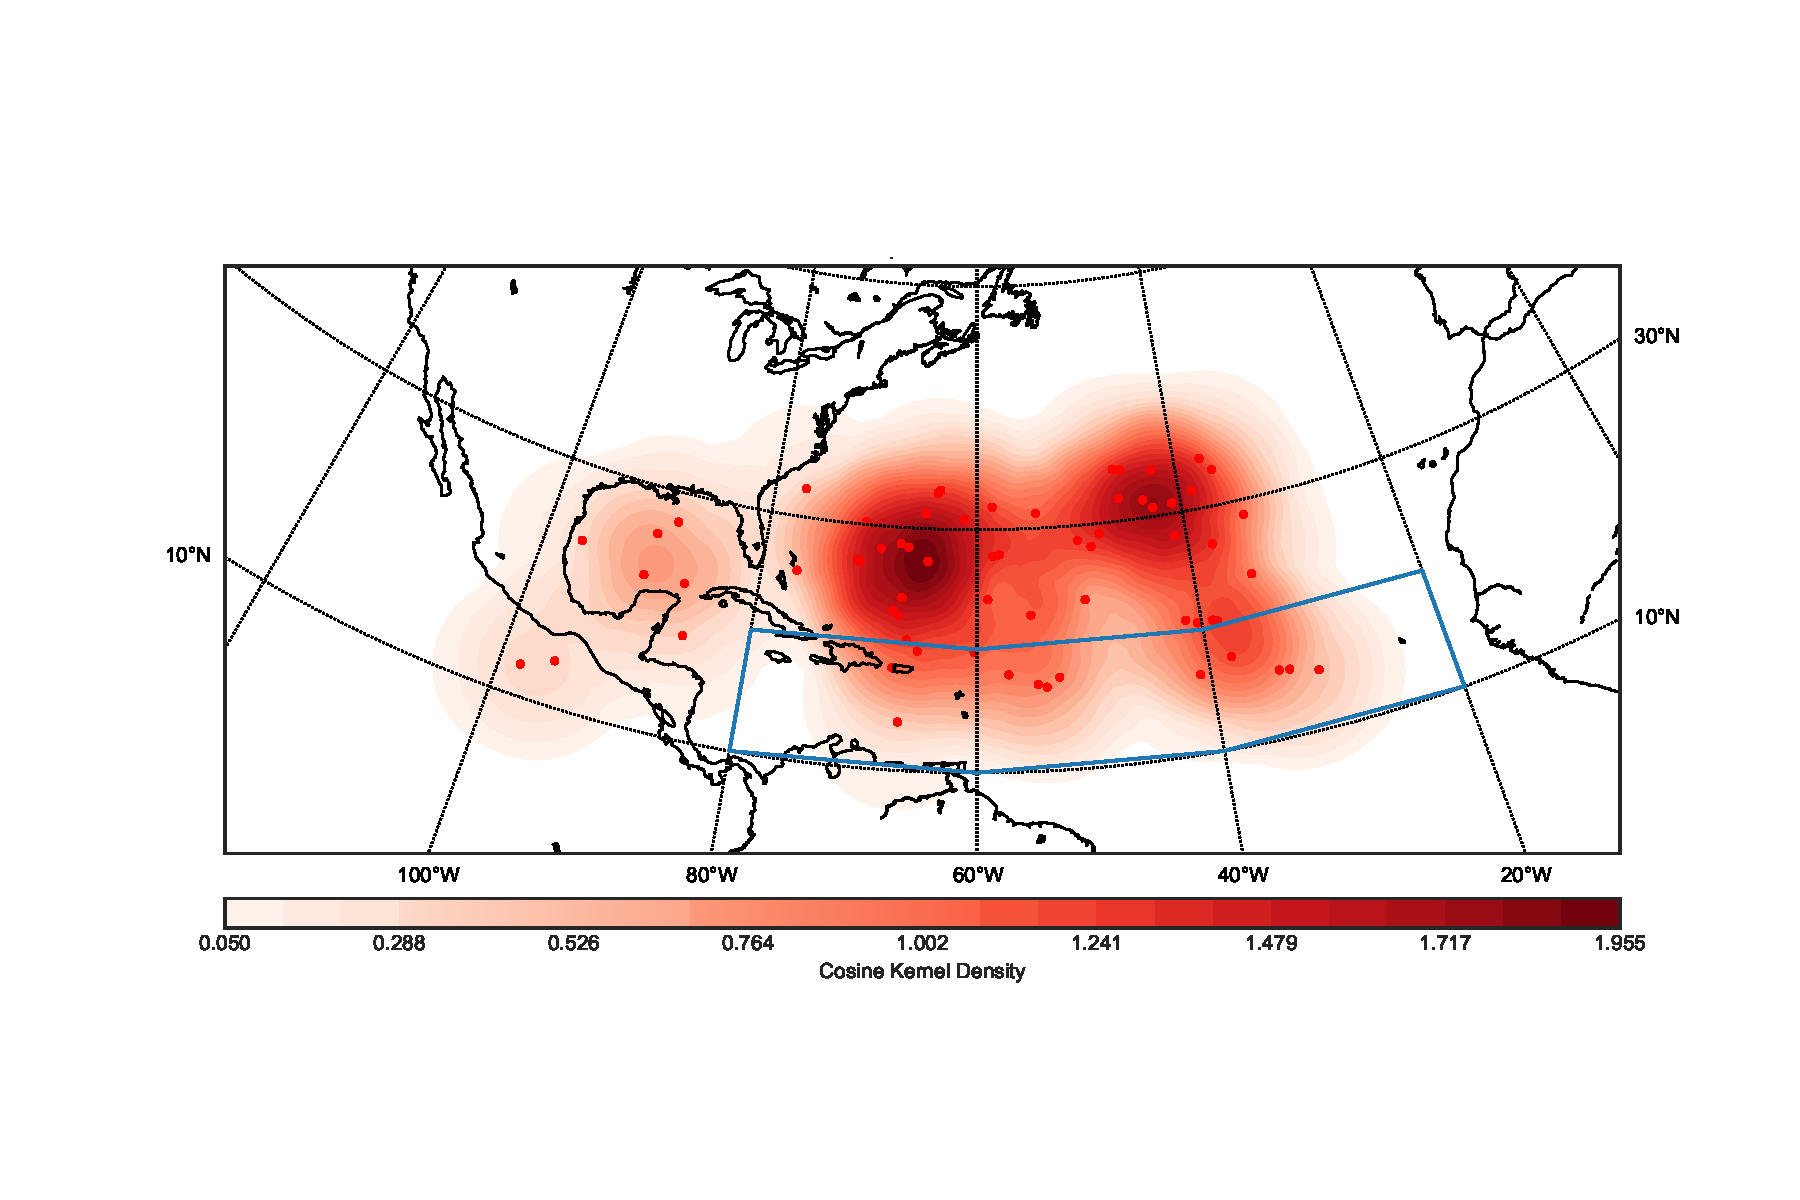
\includegraphics[width=0.8\textwidth]{img/genesis_plot_temdif15.pdf}
	\caption{Genesis spots and density for temdif = 1.5. Using param\_id = 189.}
\end{figure}

%---------------------------------------------------------------------------
% Track Matching

\chapter{Further matched tracks plots}\label{sec:matching-appendix}

\begin{figure}[ht]
	\centering
	\includegraphics[width=\textwidth]{img/B_matching_plot_reasonable_amw_ref_01_tc102806_param_id149_cat3.png}
	\caption{Matching plot of TC (102806), Category 3.}
\end{figure}
\begin{figure}[ht]
	\centering
	\includegraphics[width=\textwidth]{img/B_matching_plot_reasonable_amw_rm_10_tc37539_param_id149_cat2.png}
	\caption{Matching plot of TC (37539), Category 2.}
\end{figure}
\begin{figure}[ht]
	\centering
	\includegraphics[width=\textwidth]{img/B_matching_plot_reasonable_amw_ref_03_tc101658_param_id149_cat2.png}
	\caption{Matching plot of TC (101658), Category 2.}
\end{figure}

%---------------------------------------------------------------------------
% Lifetime

\chapter{Lifetime dependence on the warm core criterion}\label{sec:lifetime-appendix}

\begin{figure}[ht]
	\centering
	\includegraphics[width=0.7\textwidth]{img/lifetime_for_different_temdif.eps}
	\caption{Histogram showing the number of TCs with a certain lifetime in days.}
\end{figure}

 
 
%---------------------------------------------------------------------------
% Symbols

\chapter*{Nomenclature}\label{chap:symbole}
 \addcontentsline{toc}{chapter}{Nomenclature}
 
\section*{Acronyms and Abbreviations}
\begin{tabbing}
 \hspace*{1.6cm}  \= \kill
 ETH \> Eidgen\"{o}ssische Technische Hochschule \\[0.5ex]
 TC \> Tropical cyclone \\[0.5ex]
  TD \> Tropical depression \\[0.5ex]
 TS \> Tropical storm \\[0.5ex]
 DWD \> German Weather Service\\[0.5ex]
 MPIM \> Max Planck Institute for Meteorology\\[0.5ex]
ICON \> Icosahedral Nonhydrostatic Model developed by the DWD and the
MPIM\\[0.5ex]
SST \> sea surface temperature\\[0.5ex]
SLP \> sea level pressure\\[0.5ex]
MDR \> main development region  \\[0.5ex]
\end{tabbing}

%---------------------------------------------------------------------------
